% !TEX root = diplomarbeit.tex
\chapter{Firmware}
\renewcommand{\kapitelautor}{Autor: Christina Bornberg, Lucas Ullrich}

%%%%%%%%%%%%%%%%%%%%%%%%%%%%%%%%%%%%%%%%%%%%%%%%%%%%%%%%%%%%%%%%%%%%%%%%%%%%%%%
\section{Allgemeine technische Planung}

  \subsection{Konvention}
  In der Arbeit wird folgende Konvention festgelegt. Die z-Achse ist die Höhe, die y-Achse ist vorwärts und rückwärts und die x-Achse ist Seitwärts.

  % BILD %

  \subsection{Multicopter}
  Multicopter gehören zu der Luftfahrzeuggattung Hubschrauber. Sie starten senkrecht und können durch den Antrieb der Rotoren Neigung erzeugen. Durch diese Neigung kann der Hexacopter nach vorne, zurück, nach links und nach rechts fliegen. Durch die Rotoren, bei denen sich abwechselnd einer nach links und einer nach rechts dreht, kann sich der Hexacopter zusätzlich um seine Hochachse drehen.

    \subsubsection{Funktion}
    Ein Multicopter besteht im Normalfall aus folgenden Komponenten:
    Dem Empfängermodul, dem DJI NAZA-M Flightcontroller sowie der Multicopterhardware (Rotoren, Motoren, Gestell und Leistungselektronik). Der Empfänger des Multicopters kann von einem Sender Steuersignale empfangen und aufgrund der empfangenen Steuersignale Soll-Werte für die Motoren berechnen, um den Multicopter auf die entsprechende Höhe bzw. entsprechende Geschwindigkeit in x, y oder z Richtung zu bringen.

    % BILD Funktion Blockschaltbild (Dokument) %

    \subsubsection{Erweiterte Funktion}
    Im Rahmen dieser Diplomarbeit wurden die üblicherweise verwendeten Teile um vier weitere Komponenten erweitert, um einen automatischen Flug zu gewährleisten: Pixycam, Ultraschallsensor, WLAN Modul und ein Mikrocontroller. Pixycam und Ultraschallsensor sind dafür verantwortlich, die Daten für die Berechnung der augenblicklichen Position des zu bestimmen. Im Mikrocontroller läuft ein Algorithmus, der aus diesen empfangen Daten die Position überprüft. Wenn der Wert vom optimalen Bereich abweicht, werden die Steuersignale abgeändert. Durch das Wlan-Modul bekommt der Mikrocontroller die Information, durch wie viele Marker der Weg definiert ist und welcher Farbcode der letzte ist, auf dem die Landung erfolgt.

    % BILD %

    \subsubsection{Multicopter Arten}
    Es gibt verschiedene Arten von Multicoptern.
    Je nachdem wie viele Rotoren in einer Ebene liegen, setzt sich der Name zusammen.
    Die bekannteste Art ist der Quadrocopter, welcher 4 Rotoren besitzt. Weiters gibt es Hexacopter mit 6 und Octocopter mit 8 Rotoren. \cite{GrundlagenMulticopter}

    Der Flightcontroller DJI Naza-M lite unterstützt verschiedene Konfigurationsarten von Quadrocoptern und Hexacoptern. Hierzu zählen + und x Konfiguration für den Quadrocopter. Beim Hexacopter gibt es die Varianten +, x, reverse Y und Y. Diese werden im nächsten Abschnitt genauer beschrieben. \cite{NAZA_Konfig}

    \subsubsection{Konfiguration}
    Grundsätzlich gibt es 2 Arten einen Multicopter zu Konfigurieren. \cite{GrundlagenMulticopter}
    Einerseits die +- beziehungsweise I-Konfiguration, andererseits die x- beziehungsweise H-Konfiguration. Weiters gibt es die weniger verbreitete Y-Konfiguration. Dabei geht es um die Ausrichtung und die damit verbundene Fluglage.

    Für diese Diplomarbeit wurde die + Konfiguration für Hexacopter gewählt.

    Wie auf folgender Grafik ersichtlich ist, gibt es nach links und nach rechts drehende Rotoren. Die rot gekennzeichneten Arme geben an, wo die Vorderseite des Multicopters ist. Bei der Y-Konfiguration sind die blau Makierten Propeller oben, die Roten unten.

    % BILD mit 4, 6, 8 in + bzw x %

  \subsection{Mögliche Anwendungsgebiete}
  Multicopter finden in vielen Bereichen Anwendung. \cite{copterAnwendung}
  \begin{itemize}
    \item Fotographie und Videos / Filmindustrie / Anfertigen von hoch aufgelösten Luftbildkarten
    \item Multicopter als Hobby / Kunstflug
    \item Lagerhallen und Logistik / Bestands- und Inventaraufnahmen im Straßenbau
    \item Forschung / Schwarmverhalten
    \item Multicopter als Lebensretter / Rettungseinsätze / Katastrophenschutz
    \item Unterstützung der Polizei / große Menschenmengen überwachen
    \item Unbemannter Aufklärer bei Spezialeinheiten
    \item Kontrolle, Inspektion und Dokumentation von Brücken, Gebäuden, Gräben
    \item Militärische Anwendung: Spionagedrohne zur Aufklärung, Kampfdrohne zur Zerstörung, Rettungungsdrohne für Hilfsaktionen
  \end{itemize}


  \subsubsection{Steuerungsarten}

  DAS IS SCHON TEILWEISE WO ANDERS !!!!!!!!!!!!!!!!!!
  ICH KANN GRAD NICHT RECHTSCHREIBEN !!!!!!!!!!!

  Der Hexacopter wird über 4 Befehle gesteuert: \cite{GrundlagenMulticopter}

    \begin{itemize}
      \item \textbf{Aileron} auch Rollen (engl. roll) genannt, ist für die Bewegung nach Links und Rechts zuständig.
      Um diese auszuführen, werden bei der Beschleunigung nach links, die rechten Propeller stärker betrieben, umgekehrt drehen sich die auf der linken Seite befindlichen Propeller beim Flug nach rechts schneller. Durch die entstehende Neigung, fliegt der Hexacopter in die gewünschte Richtung.
      \item \textbf{Elevator} auch Nicken (engl. pitch) genannt, ist für die Vorwärts- und Rückwärtsbewegung zuständig.
      Beim nach vorne und nach hinten fliegen, werden ebenfalls die rotoren schneller betrieben, die auf der jeweils gegenüberliegenden Seite liegen.
      \item \textbf{Rudder} auch Gieren (engl. yaw) genannt, ist für die Rotation an der Hochachse zuständig.
      Um den Hexacopter um seine eigene Hochachse rotieren zu lassen, werden für eine Rotation nach rechts, die rechts-drehenden Rotoren schneller betrieben, bei der Rotation nach Links, die links-drehenden.
      \item \textbf{Throttle} reguliert die Höhe.
      Bei gleichmäßiger Ansteuerung der 6 Rotoren, kann man je nach Drehgeschwindigkeit die Höhe verändern. Der Hexacopter fliegt bei stärkerer Beschleunigung nach oben, ansonsten sinkt er. Dies wird auch als Uplift and Downfall bezeichnet.
    \end{itemize}

    U AUCH ERKLÄREN ?????????



    \subsection{Programmierung}
    Zum Programmieren des Mikrocontrollers von Microchip wurde die Programmiersprache C verwendet.
    Um die Sprache zu lernen, wurde ein sogenanntes Bootcamp als Vorbereitung für die weitere Programmierung veranstaltet.

    Das \textbf{Programmierbootcamp} leitet sich vom militärischen Bootcamp ab, in dem Rekruten ihre Grundausbildung absolvieren. Wie der Name annehmen lässt, lernt man in dieser Version die Grundlagen der Programmierung, hier im Zusammenhang mit Mikrocontrollern.

    Einfache Programme, wie ein Lauflicht oder Entfernungsmessung über einen Ultraschallsensor, wurden erstellt.
    Nach dem Initialisieren der Pins, wurde das Programm geschrieben, debuggt und getestet.
    Die Teile wurden als Grundlage für die Hexacopter Firmware genutzt.


    Durch die einfachen Programme, wurde die Entwicklungsumgebung besser kennengelernt. Die Zeit wurde auch für die Erstellung von Flussdiagrammen und das Einrichten von GitHub genutzt.

    \textbf{Codingrules}\\
    Eine weitere wichtige Aufgabe im Bootcamp war das Erstellen von Codingrules, um einheitliche Programmierung zu ermöglichen.
    Als Vorbild wurd der C STYLE GUIDE von NASA, Stand: AUGUST 1994, verwendet. \cite{NasaCGuide}

  \subsection{Tools}

    \begin{itemize}
      \item \textbf{yEd - Graph Editor}\\
      Zum Erstellen der benötigten Flussdiagramme wurde eine Desktop Anwendung namens yEd verwendet. \cite{Tool_yed}
      \item \textbf{GitHub}\\
      Zur Versionsverwaltung des Codes wurde die digitale Ablage GitHub verwendet. Durch diese ist eine gemeinsame Programmierung möglich.\cite{Tool_github}
      \item \textbf{MPLAB}\\
      MPLAB ist eine Integrierte Entwicklungsumgebung von Microchip. In dieser wurde der Mikrocontroller programmiert und anschließend compiliert. Weiters hat die Entwicklungsumgebung eine Git Funktion, wodurch die Daten ohne zusätzliches Tool vom Server herunter- beziehungsweise hinaufgeladen werden können. \cite{Tool_mplab}
    \end{itemize}

  \subsection{Positionierungssystem}

    \subsubsection{Allgemein}
    Um eine Positionsbestimmung durchzuführen, benötigt man ein Trackingsystem.
    Es gibt mehrere Verfahren, um die Position zu bestimmen: \cite{PositionAllg}
    \begin{itemize}
    \item Laufzeitverfahren (Ultraschall, GPS, optische Kreisel) ???
    \item räumliches Scanning / optische Verfahren (outside-in, inside-out)
    \item Inertialsysteme (mechanische Kreisel/Gyro, Beschleunigungssensoren)
    \item Mechanische Systeme (Gelenkarm, Seilzug, Exoskelett, Abrollen einer Kugelfläche)
    \item Magnetisches Tracking
    \item Akustisches Tracking
    \item Phasendifferenz
    \item Direkte Feldmessung (Elektromagnetisch, Erdmagnetfeld, Gravitation) ???
    \item hybride Ansätze (Kombinationen, welche genaue, aber langsame Systeme mit schnellen, ungenaueren integrieren).
    \end{itemize}

    \subsubsection{Anwendung}
    Indoor Positionierungssysteme werden derzeit vor allem zur Objekterkennung verwendet, im Umweltmonitoring, über das Detektieren von Bränden in Gebäuden,
    bis hin zum Einsatz in der Logistik, verwendet. Da es sehr viele unterschiedliche Anwendungsgebiete gibt, werden unterschiedliche Methoden. \cite{posAnwendung}

    \subsubsection{Eigenschaften der Positionsbestimmung}

    Ein Positionierungssystem kann verschiedene Arten von Informationsdaten bereitstellen. \cite{pos_eigenschaften}

    \textbf{Physische und symbolische Positionierung}\\
    Die physische Positionierung ist eine exakte Position, die zum Beispiel in einem Koordination, meist in 2-D oder 3-D Karten, bestimmt wird. Längen- und Breitengrade spielen dabei eine wichtige Rolle.\\
    Symbolische Positionierung ist die abstrakte beschreibung eines Ortes, sie wird sprachlich beschrieben, beispielsweise Küche, Garten, Dachboden.\\
    Eine physikalische Position kann auch symbolisch Beschrieben werden.

    \textbf{Relative und absolute Positionierung}\\
    Die absolute Positionierung verwendet Referenzgitter und Koordinaten. Das Paradebeispiel für absolute Ortung ist die Angabe von Längen­ und Breitengrad.   Die darauf aufsetzende Technik, die sich diese Kartographie zu Nutze macht, ist GPS. \\
    Die relative Positionierung legt ihre eigenen Rahmen vor, die auf Basisstationen oder definierten Punkten basieren. Hier wird angegeben, wie weit das Objekt entfernt ist.

    \textbf{Selbst- und fernortende Lokalisierungstechniken}\\
    Lokalisierungstechniken können weiter als selbstortend oder fernortend (engl. self­positioning/remote­positioning) klassifiziert werden. Beim optischen Tracking werden die beiden Varianten Inside-out und Outside-in genannt.\\
    Beim selbstortenden Positionierungssystem bekommt der mobile, bewegliche Empfänger die Daten von verschiedenen Sendern, die sich auf bekannten Positionen befinden. Die Lokalisation des Empfängers wird durch die gemessenen Signale ermittelt. Das Objekt kann sich selbst orten, es ist kein Netzwerk notwendig.\\
    Ein fernortendes Positionierungssystem besteht aus einem mobilen, beweglichen Sender und stationären, unbeweglichen Empfängern. Die Messdaten aller Empfänger werden gesammelt und die Position des Senders wird in der Zentrale berechnet. Hier ist ein Netzwerk notwendig, sämtliche Berechnungen werden durch eine zentrale Instanz ausgeführt.
    % BILD %

    \textbf{Genauigkeit}\\
    Die Genauigkeit gibt an, wie sehr sich gemessene und tatsächliche Position unterscheiden.

    \textbf{Skalierung}\\
    Hierbei gibt es mehrere Faktoren, beispielsweise die Anzahl der zu trackenden Objekte, die Reichweite und die benötigte Zeit.

    \textbf{Kosten}\\
    Hier gibt es Kosten im Bereich der Anschaffung des Systems und Kosten während des Betriebs.

    \textbf{Limitierung}\\
    Unter Limitierung fallen Einschränkungen und Störfaktoren. Manche Systeme haben besondere Ansprüche an ihre Umgebung.



    \subsubsection{Signalbasierte Verfahren}

    Verfahren zur Positionsbestimmung mittels Signal \cite{pos_signal_2} \cite{pos_signal_4}

    \textbf{Lateration}\\
    Bei der Lateration wird die Position mit Hilfe der Entfernungsmessung bestimmt.
    Techniken der Lateration sind TOA (time of arrival) und TDOA (time difference of arrival).\\
    Bei \textbf{TOA} werden Signale in Laufzeit gemessen. Durch die Zeitdifferenz zwischen Sender und Empfänger, kann die Entfernung mithilfe der Information, wie schnell sich das Signal fortbewegt, errechnet werden. Da sich elektromagnetische Wellen in Lichtgeschwindigkeit ausbreiten, ist die zu messende Laufzeit sehr gering. Ultraschallsignale bewegen sich vergleichsweise langsam, dies vereinfacht die Zeitmessung.
    Um schlussendlich die Position zu bestimmen, werden 3 Basisstationen benötigt, die jeweils eine Entfernungsmessung zum mobilen Objekt durchführen. Durch die 3 Entfernungen kann mittels Trilateration die Position berechnet werden.
    \\ % BILD %
    \textbf{TDOA} basiert auf der Laufzeitdifferenzmessung.
    Die mobile Sation sendet einen Zeitstempel an drei Basisstationen. Durch die Differenz der Laufzeiten, kann die Position ebenfalls mittels Trilateration bestimmt werden.
    \\ % BILD %
    \textbf{Angulation}\\
    Bei der Angulation wird die Position durch die Bestimmung von Winkeln ermittelt. \\
    \textbf{AOA} (Angel of Arrival) wird mittels Berechnung des Einfallswinkels auf ein Antennenarray umgesetzt. Bei dieser Technik werden mindestens 2 Basisstationen benötigt. Mit den Einfallswinkeln der empfangenen Signale kann die Position durch Triangulation festgestellt werden. Die Winkelbeziehungen eines Dreiecks werden dafür verwendet.
    Bei dieser Technik muss keine Synchronisation durchgeführt werden. Der Nachteil ist die benötigte komplexe Hardware.
    \\ % BILD %
    \textbf{Scene Analysis}\\
    Bei der Szenenanalyse werden Umgebungsparameter erfasst und ausgewertet.\\
    Für die Technik \textbf{Fingerprint} werden Signalstärken gemessen und als Fingerprint in einer Datenbank abgespeichert. Die Position wird dann durch den Vergleich von Fingerprints mit der Signalstärke, die bei der aktuellen Position gemessen wird, herausgefunden.
    \textbf{Proximity}\\
    Für das Verfahren Proximity wird die physische Nähe genutzt.
    Hier gibt es die Technik COO (cell of origin). \\
    Bei \textbf{COO} gibt es Basisstationen, mit bekannter Position. Die mobile Station verbindet sich mit der nächstgelegenen Basisistation. Wenn die mobile Station von mehreren Basisstationen erkannt wird, wird die Signalstärke beachtet. Diese Methode ist sehr ungenau.
    \\ % BILD %

    \subsubsection{Signalbasierte Technologien}
    \textbf{GPS (Global Positioning System)}\\
    GPS ist ein satellitengestützte Navigationssystem, das Ende der 1980er-Jahre zur globalen Positionsbestimmung entwickelt wurde. Die Nachteile des Systems sind der schlechte Empfang der Satellitensignale für indoor- Anwendungen.
    \textbf{RFID (radio-frequency identification)}\\
    RFID bezeichnet eine Technologie für Sender-Empfänger-Systeme zum automatischen und berührungslosen Identifizieren und Lokalisieren von Objekten mit Radiowellen. Ein RFID-System besteht aus einem Transponder, der sich am oder im Objekt befindet und einen kennzeichnenden Code enthält, sowie einem Lesegerät zum Auslesen dieser Kennung.
    \textbf{WPS (WLAN Positioning System)}\\
    WPS ist ein indoor Positionierungssystem, das auf WLAN basiert. Durch sogenannte  Access Points (de. drahtloser Zugangspunkt), wird die Entfernung zu Endgeräten bestimmt. Durch drei Accesspoints kann mittels Dreiecksmethode, die Position des Endgeräts ermittelt werden.
    \textbf{Ultraschall}\\
    Ein Ultraschallsensor ist Sender und Empfänger in einem. Das System basiert auf der Zeitdifferenzmessung. Er sendet ein Signal, dieses wird reflektiert und anschließend empfängt der Sensor sein eigenes Echo.
    Durch die Information, mit welcher Geschwindigkeit sich elektromagnetische sowie akustische Wellen ausbreiten, ist es möglich Entfernungen zu messen. Die Zeit, die ein Signal zum zu messenden Objekt und wieder zurück braucht, nennt man Laufzeit.

    \subsubsection{Optische Verfahren}
    Maschinelles Sehen (machine vision) beschreibt die Fähigkeit eines Computers zu sehen.
    Für einen Menschen ist es einfach, Objekte auf einem Bild zu erkennen, für Computer besteht ein Bild jedoch aus Daten, die die Graustufe beziehungsweise Farbe jedes einzelnen Pixels angeben, was die Möglichkeit des "Bildverstehens" erschwert.
    Die Auswertung erfolgt mathematisch, weswegen die Stärken von maschinellem Sehen im Bereich der Bestimmung von Farben und Graustufen, sowie der Entfernungsmessung liegen. Weiters können Maschinen, im Gegensatz zum menschlichen Auge, Infrarotlicht, Ultraviolettes Licht und Röngtenstrahlen wahrnehmen. \cite{machinevision} \cite{machinevision2}

    Es wird zwischen Objekt Erkennung (detection) und Verfolgung (tracking) unterschieden. Erkennung bezieht sich auf ein einzelnes Objekt, dass in einem Bild erkannt wird. Bei der Verfolgung werden ein oder mehrere Objekte über eine Sequenz von Bildern erkannt und somit verfolgt.
    \cite{obj_det_trak}

    \textbf{Bildverarbeitung}\\
    Die Bildverarbeitung besteht aus einer Reihe von Schritten, je nach Anwendung werden dabei manche ausgelassen.
    Der Beginn besteht aus der Bildvorverarbeitung, bei der das Bild optisch verbessert wird. Daraufhin folgt die Bildanalyse, die aus den Schritten Segmentierung, in der das Bild in Bereiche aufgeteilt wird, Merkmalsextraktion und Klassifizierung, bei der das Bild Klassen zuge besteht. \cite{Bildverarbeitung} \cite{Bildverarbeitung2}

    \textbf{Segmentierung}\\
    Beim Segmentieren teilt man ein Bild in Segmente mit gleichen Merkmalen auf.

    \subsection*{Pixelorienterte Segmentierung}
    Pixelorientierte Segmentierung wird auch Punktorientierte Segmentierung genannt. Sie basiert auf den lokalen Pixelinformationen, in Abhängigkeit der Grauwerte \cite{Seg_punkt}
    \textbf{Treshholding}\\
    Beim Treshholding, auch Schwellenwertverfahren genannt, werden Bildpunkte verschiedenen Gruppen zugeordnet. Da es eine histogrammbasierte Segmentierung wird das zu segmentierende Bild binärisiert, das bedeutet, dass jedes Pixel entweder schwarz oder weiß eingefärbt wird. Dies wird durch den Vergleich des Grauwerts oder einem anderen eindimensionalen Merkmal mit einem Schwellwert, erreicht. Der Grauwert bezieht sich nur auf die Helligkeit der Pixel, Informationen zur Farbe werden dabei ignoriert. Da dieses Verfahren bei jedem einzelne Pixel unabhängig angewendet wird, gehört es zur Pixelorientierten Segmentierung. Diese Technik benötigt wenig Rechenleistung, weshalb es in Echtzeitsystemen angewendet werden kann.

    \subsection*{Modellbasierte Segmentierung}
    Modelle, bestehend aus Pixelgruppen, werden auf Instanzen geprüft. Einfache Modelle werden mittels Template Matching oder der Hough-Transformation analysiert. \cite{Seg_modell}
    \textbf{Templatematching}\\
    Um Objekte in Bildern zu finden, müssen Information zu Struktur, Form oder Farbe vorliegen. Tempaltes, in denen diese Informationen enthalten sind, werden mit dem Bild verglichen. Anschließend wird die Region im Bild gesucht, die die größte Ähnlichkeit aufweist.
    \textbf{Hough-Transformation}\\
    Durch die Hough-Transformation können anhand der Anzahl der Pixel, die von der gesuchten Form überdeckt werden, geometrische Objekte wie beispielsweise Kreise erkannt werden. Dieses Verfahren ist sehr robust, da es auch auf verrauschten Bildern unvolsltändige oder teils verdeckte Objekte erkennt.

    \subsection*{Regionenorientierte Segmentierung}
    Hier werden benachbarte Pixel auf Gleichheit zum Startpixel geprüft. \cite{Seg_region}
    \textbf{Region Growing}\\
    Bei diesem Verfahren geht man von einem Startpixel, beziehungsweise Seed-Point aus, dieses kann entweder vom Menschen selbst oder vom Computer gewählt werden. Dieses wird mit benachbarten Pixel auf ähnliche Eigenschaften verglichen. Wenn diese Pixel genügend Ähnlichkeit aufweisen, werden sie zu einer sogenannten Region hinzugefügt, andernfalls wird das jeweilige Pixel ignoriert. Die Technologie kann in verrauschten Bildern angewendet werden.

    \subsection*{Texturorientierte Segmentierung}
    Da sich Objekte oft durch eine einheitliche Struktur auszeichnen, versucht dieses Verfahren als Homogenitätskriterium zu verwenden. Texturorientierte Segmentierung wird meist zur unterstützung anderer Methoden verwendet. \cite{Seg_textur}
    \textbf{Co-Occurrence-Matrizen}
    Um eine Texturanalyse durchzuführen, kann die Cooccurrence-Matrix, auch Grauwertübergangsmatrix genannt, verwendet werden. \cite{seg_coocc}
    Bei dieser Matrix werden die Grauwertverhältnisse der Umgebung eines Pixels beschrieben.

    \subsection*{Merkmalsextraktion}
    Bei diesem Schritt sollen Merkmale wie Kanten und Ecken erkannt werden.
    \textbf{Kantendetektion}\\

    Im menschlichen Sehen, haben Kanten eine wichtige Bedeutung. Durch sie kann ein Bild beinahe vollständig nachgebildet werden. Es gibt einige Verfahren um diese Erkennung durchzuführen.
    \textbf{Sobel Operator} Faltung des Bildes mit Hilfe einer Sobel-Matrix und anschließende Approximation der ersten Ableitung des Bildes
    \textbf{Laplace-Filter}
    \textbf{Canny Algorithmus} Zur Glättung, Einsatz eines zweidimensionalen Gaußfilters und Einsatz von gerichteten Ableitungsoperatoren. Nach der Ausdünnung der Linien, Anwendung einer Hysterese zur Erkennung ob es sich um eine Kante oder um ein Rauschen handelt.
    \textbf{Sombrerofilter} Der Sombrerofilter wird auch Laplace of Gaussian Operator und Marr-Hildreth-Operator genannt.

    \textbf{Eckendetektion}\\
    Ecken sind Punkte, in denen zwei Kanten enden, weswegen sie ebenfalls ein wichtiges Merkmal in einem Bild darstellen. Hierfür gibt es ebenfalls mehrere Verfahren.
    \textbf{Moravec´s Corner Detector} Betrachtung eines kleinen lokalen Bildfensters und Messung der Intensitätsunterschiede beim Verschieben des Fensters. Erkennung von Kanten und Ecken
    \textbf{Harris Corner Detector} Betrachtung eines lokalen Bildfensters durch Verschiebung in 4 Richtungen durch die Taylor Entwicklung

    \subsection*{Klassifikation}
    Klassifizieren ist das Zusammenfassen von Objekten zu einer Gruppe/Klasse/Kategorie. Hier gibt es beispielsweise die Klassifikation nach Farbe, Kontrast, Segmentgröße, Form oder Textur. Durch die Klassifikation soll das Erkennen von Zusammenhängen verbessert werden. Ein Objekt, bei dem alle relevanten Eigenschaften vorliegen, kann korrekt klassifiziert werden. Da in den meisten Fällen nicht alle Informationen vorliegen, wird eine Klassifizierung anhand eines Merkmalvektors, der aus einer Reihe passender Merkmale entsteht, durchgeführt. \cite{Bildverarbeitung}

    \subsection*{Verfolgen von Objekten}

    \textbf{Kalman-Filter}\\
    Kalman-Filter: Ist ein stochastischer Zustandsschätzer mit iterativer Struktur, der in Echtzeitsystemen angewendet wird unter der Annahme von normalverteilten Vorhersagen und Messungen und Vorhersage von Fehlern.

    \textbf{Optical-Flow}\\
    Optical Flow: Oberflächen erhalten eine Geschwindigkeit und eine Richtung, wobei die Bewegung von einer 3 D Szene in die 2 D Bildebene unter Berechnung eines Bewegungsvektors, der die Bewegung in Bildkoordinaten ausdrückt.

    Optical Flow:
    Dazu werden Bilder von einer Kamera an der Frontseite des Multicopters aufgenommen. Ein mitfliegender Microcontroller verarbeitet dann die Bilder mit Hilfe einer entwickelten Software. Durch einen Mustervergleich wird die richtige Situation eingeschätzt. Das Konzept funktionierte bei Translationen-Bewegung. Drehungen und größere Winkel führten jedoch zu Fehlinterpretationen. Zur Berechnung des optischen Flusses (optical flow) werden Algorithmen von Shi-Tomasi und Lucas-Kanade verwendet. Die Shi-Tomasi Algorithmen benötigen markante Punkte in Bildern, um diese wieder erkennen zu können. Auch die Lucas-Kanade-Methode verwendet die Methode der Eckenerkennung, Punkte und Ecken müssen wiedererkannt werden. \cite{opticalflow}

    \subsubsection{Optische Trackingsysteme}

    Die Lokalisierung von sich bewegenden Objekten und Bewegungserfassung

    \textbf{Pixy CMUcam5}\\
    Die Pixy CMUcam5 ist ein optisches Trackingsystem. Das Kameramodul ist in der Lage, Objekte in 7 verschiedenen Farben zu scannen, diese zu speichern und wiederzuerkennen. Daten über die Höhe und die Breite, sowie die x- und y-Position des getrackten Objektes innerhalb des Frames werden ausgegeben. Bei sogenannten Colorcodes, die sich aus zwei oder mehrfarbigen Objekten ergeben, kann die Rotation des Objektes ebenfalls ermittelt werden.

    \textbf{CMVision}
    CMVision, Color Machine Vision, ist ähnlich dem Algorithmus der Pixy
    % https://books.google.at/books?id=QHUlp1tI-JwC&pg=PT480&lpg=PT480&dq=cmvision+cmucam&source=bl&ots=xn9xZCsBk1&sig=v3GwsxR9w4SRIRX9p7uzolQWqdc&hl=de&sa=X&ved=0ahUKEwjlidqal7HLAhUGKXIKHdSuBSsQ6AEIQjAF#v=snippet&q=cmucam&f=false

    \cite{Pixy}
    \cite{Pixy_Verfahren}
    \cite{Pixy_Verfahren2}

    \textbf{Vicon}\\
    Vicon ist ein System, das mit dem Tracking-Verfahren Motion Capture (Bewegungs-Erfassung) arbeitet.
    Mehrere Kameras werden in einem Raum verteilt. Jede Kamera besitzt einen Infrarotfilter und Infrarot-LEDs. Die Lampen senden infrarotes Licht aus, dieses wird an Markern, die sich auf dem zu trackenden Objekt befinden, reflektiert. Mithilfe einer Software kann dadurch eine dreidimensionale Karte erstellt werden.
    \cite{Vicon}

  \subsection{Konzepte}
  Die verschiedenen Positionierungsarten wurden verwendet, um Konzepte für die Navigation zu entwickeln.

    \subsubsection{Aufgabenstellung}
    Damit der Hexacopter autonom durch den Raum navigieren kann, benötigt er ein Positionierungssystem.

    \subsubsection{Funkbasiertes Tracking}

      \textbf{Tracking mittels Time of Arival}\\

      Mithilfe der Laufzeitmessung können Objekte, die mit einem Empfänger ausgestattet sind, geortet werden. Dafür wird die Zeit die ein Signal vom Sender zum Empfänger benötigt gemessen. Das Signal ist eine elektromagnetische Welle, die sich im Vakuum in Lichtgeschwindigkeit ausbreitet. Die gemessene Laufzeit wird mit der Lichtgeschwindigkeit multipliziert, damit kann die Entfernung berechnet werden.

      Bei diesem Konzept, soll durch die benützung sogenannter Pseudolites (Gefälschte Sateliten) eine Art lokales GPS erschaffen werden.

      Das System besteht aus 3 Sendern, die signale Schicken und einem Empfänger, der sich im Hexacopter befindet.
      Durch das Senden eines Signals von jedem Pseudolite zum Empfänger, können 3 Distanzen berechnet werden.
      Aus diesen 3 Distanzen und der bekannten Koordinaten der Pseudolites, wird die augenblickliche Position mittels Trilateration des Hexacopters berechnet.

%\[
%      Distanz 1 = (x1 - x)^2 + (y1 - y)^2 + (z1 - z)^2
%      Distanz 2 = (x2 - x)^2 + (y2 - y)^2 + (z2 - z)^2
%      Distanz 3 = (x3 - x)^2 + (y3 - y)^2 + (z3 - z)^2
%\]

      Distanz ... ist die durchgeführte Messung\\
      x1, y1, ... z2, z3 ... sind die staatischen Koordinaten von den Pseudolites \\
      x, y, z ... werden durch die Lösung dieses quadratischen Gleichungssystems ermittelt \\

      Beim lösen der Gleichung erhält man 2 Schnittpunken. Dies ergibt sich aus der logischen Schlussfolgerung, dass die Oberflächen 3er verschmolzener Kugeln 2 Schnittpunkte haben.
      Wenn die Pseudoliten am Boden anbringt, liegt eine der beiden Lösungen oberhalb und die 2. Lösung unterhalb des Bodens, womit man einfacherweise, die Lösung mit der negativen Z-Koordinate ausschließen kann.

    \subsubsection{Optisches Tracking}
    % Aufgrund der Komplexität einer signalbasierten

  \textbf{Kamerasystem im Raum}\\

  Beim optischen Tracking mit Markern wird mit Kameras gearbeitet, welche aktive (also ein Signal emittierende) oder passive Marker an den zu erfassenden Personen oder Gegenständen verfolgen.

  Für ein fernortendes Positionierungssystem, werden Kameras in einem Raum verteilt.
  Sowohl Tische und Kreuzungen als auch der Hexacopter sind mit Markern versehen. Die einzelnen Komponenten werden vom Kamerasystem erfasst und anschließend wird eine Karte erstellt. Diese Karte besitzt, wie ein Koordinatensystem Längen und Breitengrade.

  Der Hexacopter wählt seine Route, die er mittels Position der Kreuzugen und Tische berechnet.

  Durch das Trackingsystem kann die Position des Hexacopters getrackt werden. Somit wird kontrolliert, ob er sich auf der richtigen Route befindet.

  Anhand der Markerbewegungen in den einzelnen Kamerabildern kann mittels Triangulation die Position der Marker in 3D berechnet werden.

  \textbf{Linien}\\
  Bei einem selbstortenden Positionierungssystem sind Sensoren auf dem sich bewegenden Objekt angebracht.
  Der Hexacopter trackt eine Linie, die Kamera ist am Hexacopter befestigt
  Zunächst wurde ein Konzept mit Linien erstellt. Der Hexacopter folgt einer einfarbigen Linie, bis er zu einer Kreuzung kommt, nun ist seine Aufgabe, die nächste Linie zu finden, um seinen Weg zum Ziel zu finden.

  Vorteile: Der Hexacopter kann die Linie nur schwer verlieren
  Nachteile: Das verwendete Kamerasystem ist nicht in der Lage eine Linie zu tracken.


  \textbf{Farbcode pro Wegabschnitt}\\
  Durch die Verwendung der Pixy CMUCam5 ergibt sich die Möglichkeit, Farbobjekte, die eine oder mehrere Farben haben, zu scannen.

  Bei diesem Konzept bekommt der Mikrocontroller Informationen zu den Farbobjekten pro Wegabschnitt. Vom Start bis zur ersten Kreuzung verwendet er eine Farbinformation, die aus einem Colorcode besteht. Jedes Farbobjekt auf diesem Weg, hat die selben 2 Farben. Durch diese Technik hat der Administrator des Systems weniger Aufwand.

  Version 1: 1 ColorCode pro Wegabschnitt

  Vorteile:
  - (kein Problem, wenn ein Farbobjekt nicht mitgetrackt wird)

  Nachteile:
  - die Korrektur der Rotation ist komplizierter, da zuerst über das Koordinatensystem der Kamera herausgefunden werden muss, welches Farbobjekt am nächesten zu y = 0 ist.
  - Weiß nicht, ob das Nächste wirklich das Nächste ist oder ein Fehler

  \textbf{Farbcodes variieren}\\
  Das gewählte System wird ebenfalls mittels 2-farbiger Codes umgesetzt.

  Erklärung: Jedes Farbobjekt hat einen ColorCode

  Vorteile:
  keine großartigen Kosten neben Copter und Server
  Rechnung am Hexacopter
  - relative Position kann besser bestimmt werden
  - kennt das Ende des Weges und muss daher nicht herausfinden, wann der Weg zu ende ist und die Landeplattform vor ihm ist

  Nachteile:
  - (Probleme, sollte ein Farbobjekt nicht erkannt werden)
  - Mehr Aufwand bezüglich auflegen der Farbobjekte -> man muss eine Reihenfolge beachten. Dadurch müssen auch mehrere Daten vom Server geschickt werden. => die Farbinformation ist länger, da jedes einzelne Objekt eingetragen werden muss.



  \textbf{Tracking mittels Infrarot}\\
  Um das System auch ohne entsprechende Lichtverhältnisse durchführen zu können, besteht die Möglichkeit einen Infrarotfilter an der Pixycam anzubringen und die Wegpunkte mittels Infrarotlampen zu makieren.

  Vorteile:
  System funktioniert ebenfalls im Dunkeln.
  Nachteile:
  Jeder Tisch benötigt einen Stromanschluss.
  Die Wartung ist aufwändiger.
  Komplexer für den Administrator - wo ist welcher Infrarotsender (Für den Menschen nicht sofort ersichtlich)


  \subsubsection{Das gewählte Konzept}

  Das geählte Konzept ist ein optisches Trackingsystem, bei dem die Farbcodes variieren.

  Um die Höhe zu messen wird eine einfache Entfernungsmessung mittels Ultraschallsensor durchgeführt.

  Das System wurde auf die oben genannten Eigenschaften analysiert:

  \textbf{Physische und symbolische Positionierung}\\
  Die Positionierung erfolgt physisch. Durch die Pixy kann die tatsächliche Position ermittelt werden.
  Zum Besseren verständnis, wir die Positionen ebenfalls symbolisch beschrieben. Es werden die Namen Base, für die Küche beziehungsweise den Stützpunkt, Weg für die Route aus Colorcodes und Tisch, für die Landeplattform, auf der der Hexacopter landen soll, verwendet.

  \textbf{Relative Positionierung}\\
  Das gewählte System gestaltet sich relativ, da der Hexacopter seine Position relativ zu Farbobjekten bestimmt.

  \textbf{Selbstortendes Positionierungssystem}\\
  Das Positionierungssystem ist selbstortend. Die am boden liegenden Farbobjekte werden von der Pixy getrackt und die daraus entstehenden Daten verarbeitet. Der Hexacopter kann ohne externe Einflüsse navigieren und ist somit unabhängig.

  \textbf{Genauigkeit}\\
  Da das System mittels optischem Tracking umgesetzt wird, ist die Genauigkeit sehr hoch.

  \textbf{Skalierung}\\
  Das System ist beliebig Skalierbar, da es auf Farbcodes basiert. Es besteht die Möglichkeit, beliebig viele Farbcodes dem Weg hinzuzufügen oder wieder wegzunehmen. Die Routen sind im Adminbereich hinterlegt und müssen, je nach dem, wie der Administrator die Farbcodes legt, diese auch mitverändern. Im System gibt es aus Testgründen eine Grenze von 20 Farbcodes, diese kann aber einfach verändert werden.

  Die Pixy CMUcam5 ist in der Lage 135 Objekte pro Frame zu tracken. Unser System ist selbstortend, dewegen interessiert sich der Hexacopter nur für ein Objekt pro Frame. \cite{PIXY_Porting_Examplecode}

  Das System ist, wegen des Ultraschallsensors auf eine Höhe von 3 Metern begrenzt. Im System ist eine Maximalhöhe von 220m über dem Boden und 120m über einem Tisch hinterlegt.

  \textbf{Kosten}\\
  Da  die Positionierung auf einer Kamera mit Farbcodes, einem Ultraschallsensor, einem Mikcrocontroller und einem WLAN fähigen Gerät basiert, beschränken sich die Kosten auf wenige Hundert Euro

  \textbf{Limitierung}\\
  Die Pixy CMUcam5 muss zuvor gespeicherte Farben wiedererkennen, die Lichtverhältnisse müssen daher optimal sein.
  Objekte müssen eine Mindestensgröße von 4x1 Pixel in einem Frame ausmachen. Die Pixycam kann Objeke, laut Angaben der Website, über Kilometer tracken, wenn diese groß genug sind. Beispielsweise kann ein Objekt in Ping-Pong Ball Größe aus einer Entfernung von etwa 3 Metern gescannt werden.
  \cite{Pixy}

  Das System kann sowohl Indoor als auch Outdoor angewendet werden.

  Der verwendete Ultraschallsensor misst die Entfernung mit einer Auflösung von 3mm. Er eignet sich für den Bereich zwischen 2cm und 3m.
  \cite{Ultrasonic}

  \subsection{Tischplan}
  Das Konzept Tischplan beschreibt den Aufbau / die Infrastruktur des Restaurants. Welche Komponenten benötigt werden und wo diese platziert sind.
  Um eine vorgegeben Route fliegen zu können muss der Multicopter einen Routenplan vorgegeben bekommen, in diesem sind die einzelnen Markierungspunkte enthalten, welche der Multicopter auf seinem Weg zum Tisch überfliegt.

  Komponenten des Restaurants, hier kommt die symbolische Positionierung zum Einsatz.

  \textbf{Küche}\\
  Die Küche beschreibt den Bereich, in dem der Kellner interagiert. Hier befindet sich eine Base, dies ist eine Plattform, die mit einem Farbcode ausgestattet ist. Auf ihr steht der Hexacopter und wartet auf die Beladung des auszuliefernden Cupcakes und den Befehl, loszufliegen.
  Das Admin Interface und der Server stehen ebenfalls in der Küche, über diese Komponenten bekommt der Hexacopter Befehle. Die Routen sind im Admin Interface hinterlegt.

  \textbf{Weg}\\
  Der Weg besteht aus sich abwechselnden 2 farbigen Codes. Die Teile zwischen Tischen und Kreuzungen, werden als Wegabschnitt bezeichnet.

  \textbf{Tisch}\\
  Auf einem Tisch befindet sich, wie in der Küche eine Plattform, die mit einem Farbcode versehen ist. Hier landet der Hexacopter, wartet 30 Sekunden lang und fliegt danach den Weg zurück zu seiner Base. In den 30 Sekunden soll der Cupcake entnommen werden. Weiters befindet sich ein iPad auf jedem Tisch. Durch dieses enthält jeder Tisch seine eigene ID und dazugehörige Route. Bestellungen können somit einem Tisch zugewiesen werden.

  % Bild vom Ablauf %%%%%%%%%%%%%%%%%%%%%%%%%%%%%%%%


  \subsection{Flussdiagramme}
  Für einen besseren Überblick über die einzelnen Programme und deren geforderten Funktionen wurden einzelne Flussdiagramme des gesamten Prozesses erstellt.
  Diese dienen nachfolgend als Orientierung beim Programmieren der einzelnen Funktionen.

  \begin{figure}[tbh]
    \begin{centering}
      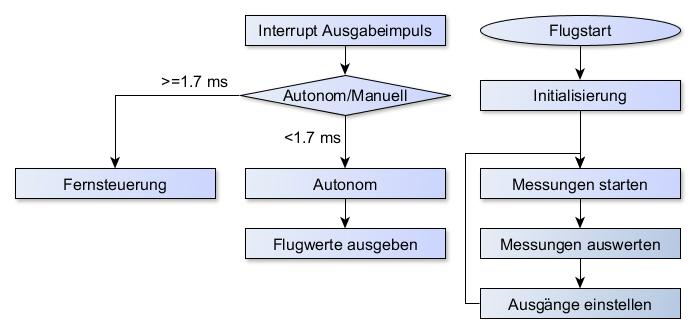
\includegraphics[width = \textwidth]{Bilder/Flussdiagramm}
    \par\end{centering}
    \caption{Flussdiagramm des Gesamtablaufs}
    \label{Flussdiragramm}
  \end{figure}

  Für die weiteren Programmteile wurden jeweils noch detailliertere Flussdiagramme erstellt.

  \subsection{Aufbau des Programms}

  % Erklärung, wer was Aufruft %





%%%%%%%%%%%%%%%%%%%%%%%%%%%%%%%%%%%%%%%%%%%%%%%%%%%%%%%%%%%%%%%%%%%%%%%%%%%%%%%
\section{Navigation}

  \subsection{Technische Planung}

    \subsubsection{Frames}

    Ein Frame hat die Größe von xxx

    Ein Frame entsteht bei jeder Messung der Pixy CMUcam5. Der Frame hat eine Breite von 319 und eine Höhe von 199 Pixel. Die Koordinate (0/0) befindet sich in der linken oberen Ecke.

    Bild 1 beschreibt den alten Frame, Bild 2 den aktuellen. Die Position des Objektes, beschreibt die zentralen x und y Positionen des Frames. Die Differenz entsteht aus den Positionen des Objektes im alten und neuem Frame. Das Objekt soll in den Bereich zwischen X_MIN und X_MAX, beziehungsweise Y_MIN und Y_MAX gelangen.

    % BILD VON LUCAS %

    \subsubsection{Aileron}

    Die Beschleunigung auf die Seiten links und Rechts

    Anhand des aktuell getrackte Colorcodes werden die Seiten links und rechts korrigiert.

    \subsubsection{Elevator}
    Vorwärts- und Rückwärtsbewegung: Die Vorwärtsbewegung muss auf einer konstanten Position gehalten werden. Beim Endpunkt wird die Geschwindigkeit der Vorwärtsbewegung auf 0 gesetzt werden. Im Idealfall muss eine Rückwärtsbewegung gar nicht durchgeführt werden, nur, wenn der Multicopter über das Ziel hinausschießt.

    \textbf{Das Weiterschalten auf den nächsten Bodenmarker}\\
    Der Algorithmus zielt immer auf den Marker, der sich am nächsten zum Nullpunkt an der y-Achse befindet. Er trackt den Ersten, bis er den zweiten erkennt, diesen verfolgt er wieder, danach kommt der dritte dran, diese Routine läuft, bis der letzte Colorcode erreicht ist. Welcher Marker der Zielmarker ist, wird durch die größe eines Arrays erkannt. Dieses wird mit den Daten, die im Admin-Interface hinterlegt sind und im Endeffekt vom Wlan-Modul empfangen werden, befüllt.

    \subsubsection{Rudder}

    Mithilfe der Rudder Funktion muss der Winkel auf die aktuelle Positionsmarkierung ausgerichtet werden.

    \subsection*{Darstellung negativer Zahlen im Binärsytem}

    Für die Rotation werden die Grundlagen negativer binärer Zahlen benötigt.

    \textbf{Binäre Zahlen ohne Vorzeichen}\\
    0000 0000 = 0, 1111 1111 = 255
    \textbf{Binäre Zahl mit Vorzeichen}\\
    Ein Bit wird für das Vorzeichen verwendet.
    0000 0001 = 1 -> 1000 0001 = -1,
    0111 1111 = 127 -> 1111 1111 = -127
    \textbf{Einerkomplement}\\
    Beim Invertieren aller Bits entsteht eine negative Zahl
    0000 0000 = "+0" -> 1111 1111 = "-0"
    0111 1111 = 127 -> 1000 0000 = -127
    \textbf{Zweierkomplement}
    0000 0001 = 1 -> 1111 1111 = -1
    0000 0010 = 2 -> 1111 1110 = -2
    0111 1111 = 127 -> 1000 0001 = -127
    \textbf{Bilden des Zweierkomplements}
    Beispiel: 0111 1111 = 127
    Die Binäre Zahl wird invertiert (1000 0000) und mit 1 addiert.
    Das Ergebins lautet: 1000 0001 = -127
    Beispiel: 1000 0000 = 128 (im Komplement)
    Die binäre Zahl wird mit 1 subtrahiert (0111 1111) und danach invertiert.
    Das Ergebnis lautet: 1000 0000 = 128 = -128

    % Bild von Rotation %

    \subsubsection{Throttle}
    Über den Ultraschallsensor erfährt der Hexacopter, wie hoch er fliegt, wenn er seine maximale Flughöhe erreicht hat, soll er seine Antriebskraft nicht weiter erhöhen. Dadurch korrigiert er seine Höhe bei jedem Aufruf der Funktion und eine Änderung des Gewichts, wird ausgeglichen. Der entnommene Cupcake am jeweiligen Tisch soll daher keine Probleme erschaffen.

  \subsection{Umsetzung}

    \subsubsection{Vergleichen der Frames}
    Für den Vergleich des aktuellen mit dem letzten Frame, werden zwei \glslink{Struktur}{Strukturen} verwendet, die über folgende Mitglieder verfügt. \cite{Structs}
    \begin{itemize}
      \item \textbf{num} ist die ID des getrackten Colorcodes, er besteht aus einer zweistelligen Zahl.
      \item \textbf{pos\_x} ist die X-Position des Colorcodes. Der Wert bezieht sich auf das Zentrum des Objektes.
      \item \textbf{pos\_y} ist die Y-Position des Colorcodes. Der Wert bezieht sich auf das Zentrum des Objektes.
      \item \textbf{height} ist die, vom Ultraschall übergebene Höhe.
      \item \textbf{angle} ist die Rotation des Colorcodes. Da er zweifarbig ist, kann die PIXY CMUcam5 die Rotation des Objektes feststellen.
    \end{itemize}

    Zuerst wird die ID des Colorcodes verglichen, um herauszufinden, ob das Farbobjekt das selbe wie im letzten Frame ist.
    Sollte dies der Fall sein, werden die Koordinaten x und y und die Rotation mit den Werten der älteren Struktur verglichen und in einem weiteren Struct gespeichert. Dieses wird bei den folgenden Funktionen verwendet, um anhand der Änderung zwischen zwei Frames zu überprüfen, ob der Hexacopter die richtige Geschwindigkeit hat.

    \subsubsection{Aileron, Elevator und Rudder anhand der Kameradaten}
    Durch die PIXY CMUcam5 kann die Position des Hexacopters, relativ zu einem Colorcode, festgestellt werden. Gegebenenfalls werden anschließend die Flugparameter verändert.

    \begin{figure} [tbh]
      \begin{centering}
        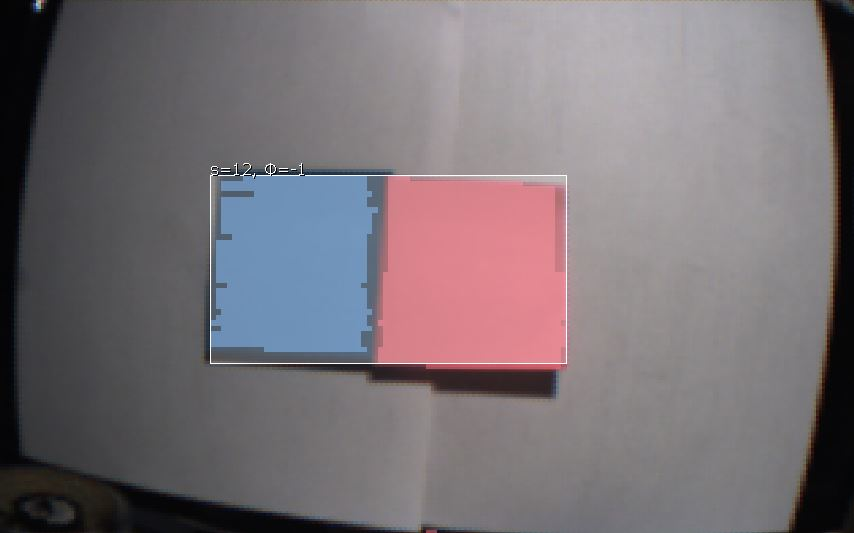
\includegraphics[width = \textwidth]{Bilder/Farbcode_erkannt}
      \par\end{centering}
      \caption{Ein erkannter Farbcode}
      \label{Farbcode_erkannt}
    \end{figure}
    Die Position wird anhand solcher Farbcodes erkannt, im Tischkonzept ist hinterlegt in welcher Reihenfolge der Hexacopter die Farbcodes suchen muss.
    Er fliegt anschließend so lange, bis er über dem aktuellen Farbcode ist, dieser also mittig im Bild ist und sucht darauf den nächsten.

    \textbf{Überprüfen von Aileron}\\
    Beim Vergleichen von Aileron wird die Veränderung an der x-Achse überprüft.

    Durch diese Funktion soll der Hexacopter mithilfe der Pixy-Daten, den Colorcode in der Mitte des Frames plazieren. An der x-Achse sind Werte zwischen 150 und 170 optimal. Der übergebene Wert ist dabei der Mittelpunkt des Colorcodes.
    Sollte die Pixycam keinen Wert in diesem Bereich erfassen, kann sie durch eine weitere Funktion namens ActAileron, die die Änderungsrate an den Flightcontroller weitergibt, die Position an der x-Achse korigieren.
    Um herauszufinden, ob der Mittelpunkt unter oder über dem optimalen Wert liegt, also der Hexacopter zu weit Links oder Rechts vom Objekt fliegt, gibt es für beide Fälle eine Abfrage.
    Um den Aileron Wert entgültig zu setzen, müssen nach der Überprüfung, ob der übergebene Wert an der x-Achse 170 über- beziehungsweise 150 unterschreitet, folgende Zustände kontrolliert werden.
    Zunächst muss der Hexacopter über die Pixycam herausfinden, ob er sich bereits in die richtige Richtung bewegt. Dafür werden die beiden Frames miteinander verglichen. Wenn der Wert zu hoch ist, muss der x-Wert im alten Frame größer als im neuen sein. Sollte er zu niedrig sein, muss der Wert im neuen Frame höher sein.
    Anderenfalls fliegt der Hexacopter auf die falsche Seite. Die Firmware reagiert darauf mit der Änderung der Pulszeit am Aileron-Pin.
    Bei der Bewegung in die richtige Richtung wird der Wert so lange in diese gesteuert, bis sich die Geschwindigkeit, gemessen in den veränderten Pixel zwischen zwei Frames, zwischen 2 Konstanten Werten befindet.

    \textbf{Überprüfen von Elevator}\\
    Elevator, die Bewegung an der y-Achse, also die Bewegung nach vorne und nach hinten, funktioniert nach dem selben Prinzip wie Aileron.

    Zuerst wird kontrolliert, ob sich der Farbcode im gewünschten Bereich befindet, in diesem Fall zwischen 90 und 110.
    Sollte der Mittelpunkt an der y-Achse nicht in diesem Bereich liegen, fliegt der Hexacopter nach vorne beziehungsweise zurück.
    Da die Route aus mehreren Farbcodes besteht, richtet sich der Hexacopter nach dem Objekt, das sich am nächsten zum Nullpunkt der y-Achse befindet. Somit probiert er die Position zentriert über dem Farbobjekt zu optimieren, bis er das nächste Farbobjekt erkennt und trackt. Das alte ist nun unwichtig, der Hexacopter bezieht sich auf das vordere Farbobjekt.

    Wie bei der Überprüfung von Aileron, gibt es auch hier zwei Konstante Werte, zwischen denen sich die Geschwindigkeit befinden soll, solange die Position optimiert wird.

    \textbf{Überprüfen von Rudder}\\
    Rudder beschreibt die Rotation um seine eigene Hochachse. Dafür wird zunächst unterschieden, ob sich der Hexacopter am hin- oder rückflug befindet, da die Rotation der Colorcodes beim Rückflug um 180 Grad gedreht werden muss.

    Die optimale Rotation befindet sich beim Hinflug zwischen -5 und 5 Grad.
    Bei einem zu niedrigen oder zu hohen Wert wird kontrolliert, ob sich der Hexacopter bereits in die richtige Richtung dreht.
    Sollte dies nicht der Fall sein, wird die Änderungsrate an die dazugehörige Funktion geschickt, die dem Flightcontroller die Information zur Beschleunigung gibt.
    Ansonsten wird die Veränderung der Pixel zweier Frames verglichen, wenn sie sich im gewünschten Bereich befindet, wird der Wert nicht geändert, bei einem zu hohen Wert, wird die Rotationsgeschwindigkeit gesenkt, ansonsten erhöht.

    Beim Rückflug soll die Rotation des Colorcodes größer als 175 oder kleiner als -175 sein.

    Die Schwierigkeit dieser Funktion, war die Rotation im negativen Bereich, da erst verinnerlicht werden musste, dass die höchste negative Zahl nicht wie im Plusbereich im Bereich unendlich liegt, sondern -1 Beträgt.


    \subsubsection{Throttle anhand des Ultraschallsensors}
    Der Hexacopter steht auf einer Landeplattform in seiner Base. Unter ihm ist ein Farbcode, diesen fokusiert er so lange, bis er den nächsten Farbcode trackt. Den zweiten Farbcode kann er erst scannen, wenn er hoch genug fliegt um an der Tischkante vorbei, den nächsten Farbcode zu scannen.

    Beim Starten fliegt er vertikal nach oben, bis er den 2. Farbcode erkennt. Um beim Start nicht abzudriften, beschleunigt er, solange er sich unter einer Höhe von 50cm befindet, mit einer Hohen Änderungsrate. Ab dieser Höhe, beschleunigt er mit einer geringeren Erhöhung der Änderungsrate, bis er die 80cm-Grenze erreicht hat.
    zwischen 80 und 120cm bleibt die Beschleunigung gleich, das führt jedoch dazu, dass der Hexacopter den oberen Rand von 120 erreichen wird, da er bis jetzt nicht gebremst wird. Sobald er über 120cm kommt, wird die Beschleunigung nach unten hin verändert. Der Hexacopter pendelt sich zwischen 80 und 120cm ein.

    Nun muss er herausfinden, ob er sich noch über dem Tisch oder schon über dem Boden befindet. Dies stellt er fest, wenn 2 hintereinanderliegende Messungen 50cm von der Vorigen abweichen. Die zweite Messung ist erforderlich, um mögliche Fehlmessungen auszuschließen.

    Wenn er nun über dem Boden fliegt, beträgt seine minimale Höhe bei 180 cm und seine maximale Höhe bei 220 cm.
    Der Hexacopter beschleunigt nach dem selben Prinzip, wie über einem Tisch. Unter 100 cm ändert erhöht er seine Beschläunigung mit einem hohen Wert. Bis 180cm beschleunigt er mit einer niedrigeren Änderungsrate. Sollte der Hexacopter über 220cm fliegen, wird die Beschleunigung durch eine negative Änderungsrate gesenkt.

    Der Hexacopter fliegt mit diesen Werten, bis er den vorletzten Farbcode erreicht hat. Da die Farbcodes in einem Array abgespeichert werden, ist die Anzahl der darin gespeicherten Farbcodes bekannt.

    Beim letzten Farbcode angekommen, also dem am Tisch liegenden Farbcode, wird ebenfalls wieder durch die Kontrolle von 2 Werten, die sich um 50cm von der vorigen Messung unterscheiden müssen, analysiert, wann sich der Hexacopter auf dem Tisch befindet. Sobald er sich am Tisch befindet, landet er, indem er die Beschleunigung mit einer negativen Änderungsrate verlangsamt. Dabei muss er sich zwischen einer vom System vorgegebenen Mindest und Maximalgeschwindigkeit befinden.

    Nach der Landung wird die Routeninformation umgekehrt, der erste Colorcode wird zum letzten, der zweite zum vorletzten und so weiter. Außerdem muss die Rotation der Farbcodes beim Rückflug um 180 Grad gedreht sein, dafür wird die Richtung als Rückflug abgespeichert. Sollte sich der Hexacopter wieder in der Base befinden, wird die Variable wieder als Hinflug gespeichert.

    Damit genügend Zeit für das herunternehmen des Cupcakes ist, verweilt der Hexacopter eine halbe Minute am Tisch, bevor er seinen Rückflug antritt.

    \subsubsection{Speichern der alten Daten}
    Die alten Daten werden gespeichert, um die Differenzen von zwei Frames zu errechnen. Der Frame mit Index 0, ist der aktuelle Frame, der Frame mit dem Index 1, der alte. Bei jedem durchlauf, werden die Werte aktualisiert.

    \subsubsection{Ausgabe der Steuersignal}
    Nachdem die Steuersignale berechnet und korrigiert wurden müssen diese an den Hexacopter ausgegeben werden. Dies muss periodisch alle $\SI{20}{\milli\second}$ geschehen.
    Der Flightcontroller erkennt jeweils die einzelnen Impulse und steuert die Rotoren entsprechend an.

    Diese Impulse werden Interrupt-gesteuert ausgegeben, der Interrupt wird von dem Gear-Pin erzeugt welcher gleichzeitig für den Flugmodus verantwortlich ist.

    \lstset{language = c}
    \begin{lstlisting}
interrupt void Isr() {
  if(CCP1IF == 1) {
    CCP1IF = 0;
    T1CONbits.TMR1ON = 0;
    SignalOut();
    NOP();
  }
  if(TMR3GIF == 1) {
    TMR3GIF = 0;
    ModeCheck();
    SignalOut();    /* initial call after remaining break to 20 ms
                     * starts with Aileron (needs to be set in last
                     * case statement, case 0) following delays will
                     * be processed by the previous routine */
    pulsecounter++;
  }
}

void SignalOut(void) {
  switch(pin_out) {
    case 'A': {
      A = 1;
      Delay(a_actors[0].aile);
      pin_out = 'E';
      break;
    }case 'E': {
      A = 0;
      E = 1;
      Delay(a_actors[0].elev);
      pin_out = 'T';
      break;
    }
    \end{lstlisting}
    Die weiteren Signale (Throttle und Rudder) werden auf die gleiche Weise ausgegeben.
    Die Delay-Funktion stellt die Compare-Einehit so ein, dass nach der gewünschten Pulsdauer des Ausgangs ein Interrupt hervorgerufen wird.

%%%%%%%%%%%%%%%%%%%%%%%%%%%%%%%%%%%%%%%%%%%%%%%%%%%%%%%%%%%%%%%%%%%%%%%%%%%%%%%
\section{Objekterkennung}

  \subsection{Technische Planung}

  \subsection{Umsetzung}

  \subsection{Herausforderungen und Lösungen}

%%%%%%%%%%%%%%%%%%%%%%%%%%%%%%%%%%%%%%%%%%%%%%%%%%%%%%%%%%%%%%%%%%%%%%%%%%%%%%%
\section{Sicherheit}

  \subsection{Technische Planung}

Sicherheitskonzepte

Beim Konzept Sicherheitsmaßnahmen geht es grundsätzlich um die Sicherheit von Mensch, Umgebung und dem Multicopter selbst. Hier werden mögliche Fehler mit Anlehnung an FMEA ("Fehlermöglichkeits- und -einflussanalyse" / "Auswirkungsanalyse") analysiert. Dieses Konzept ist ein rein schriftliches Konzept.


  \subsection{Umsetzung}

\begin{table}[H]
\centering
\begin{tabular}{|r|l|p{7cm}|c|}
\hline \# & Bezeichnung & Beschreibung & Bewertung \\\hline
\hline 1 & PL Michael Springsits & Projektleiter vieler schulischer Projekte, zeigt stets Neugier für neuartige Technologien und programmiert leidenschaftlich. & + \\
\hline 15 & crypt-drive team & Zwischenmenschliche Probleme können das Projektklima negativ beeinflussen.  & - \\\hline
\end{tabular}
\caption{Beschreibung der Umfelder}
\end{table}


%%%% WAS PASSIERT DANACH ????


%%%%%%%%%%%%%%%%%%%%%%%%%%%%%%%%%%%%%%%%%%%%%%%%%%%%%%%%%%%%%%%%%%%%%%%%%%%%%%%
\section{Systemausfall}

  \subsection{Technische Planung}

  \subsection{Umsetzung}

%%%% WAS PASSIERT DANACH ????
